\newpage
\section {Relatório de Outubro}

\subsection{Propostas para o mês:}
\begin{enumerate}
    \item Adicionar customização:
    \begin{itemize}
        \item Criar um menu para montagem de decks (baralhos).
        \item Adicionar mais cartas, o suficiente para criar mais de um baralho totalmente diferente uns dos outros.
    \end{itemize}

    \item Personalização \textit{in game}: 
    \begin{itemize}
        \item Incluir estágios/fases novas para o jogo, com novos desafios e oponentes.
        \item Adicionar um método para adquirir novas cartas conforme completa desafios e vence adversários. 
    \end{itemize}
\end{enumerate}

\subsection{Atividades Realizadas:}

\subsubsection{Jogador e criação do baralho}

Durante esse mês, foi decidido que seria melhor fechar um pouco mais o escopo. Algumas \textit{features} não poderiam ser entregues até o fim do ano, então a meta se tornou completar o básico para uma partida do jogo. Visto isso, a classe jogador foi implementada com as principais funções de compra, criação de \textit{deck} a partir de um arquivo json e funções secundárias de \textit{getters}, \textit{setters} e liberar memória. 

\begin{figure}[htbp]
    \centering
    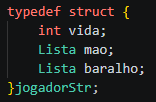
\includegraphics[width=1.0\textwidth]{jogador-estrutura.png}
    \caption{Estrutura da classe jogador.}
\end{figure}

\begin{figure}[htbp]
    \centering
    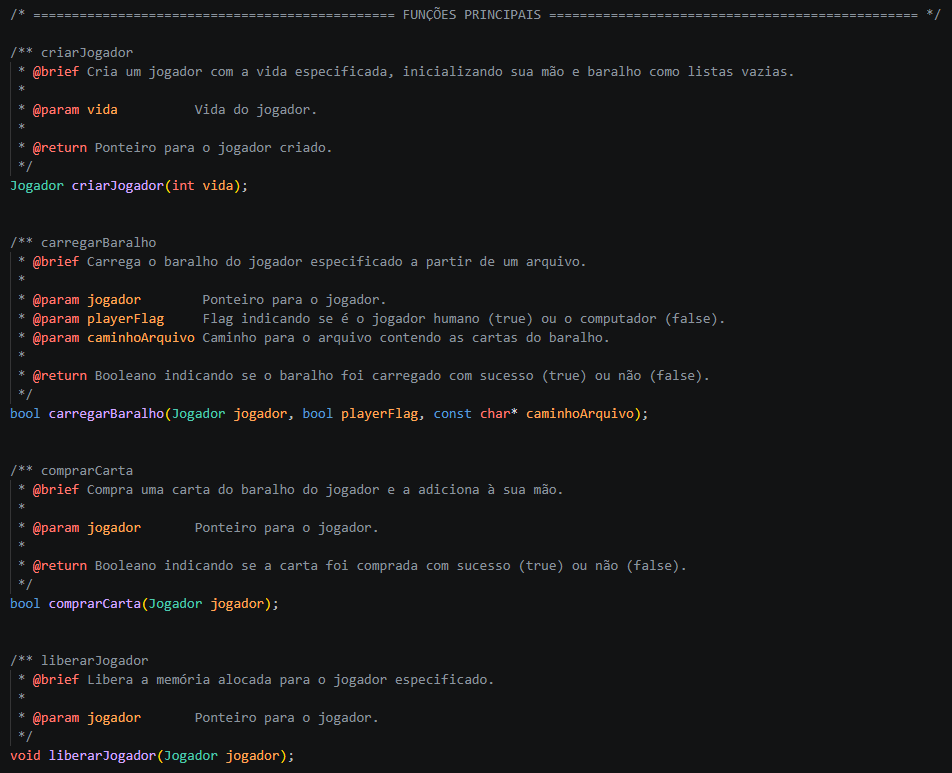
\includegraphics[width=1.0\textwidth]{jogador-funcoes1.png}
    \caption{Funções principais.}
\end{figure}

\begin{figure}[htbp]
    \centering
    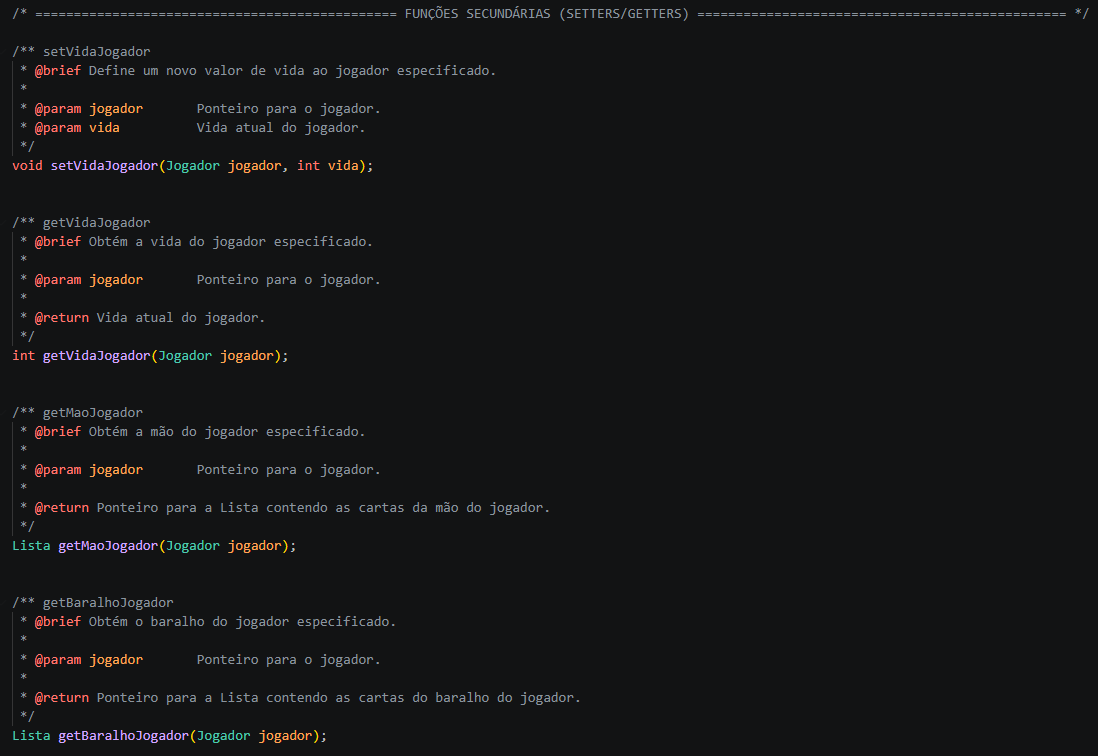
\includegraphics[width=1.0\textwidth]{jogador-funcoes2.png}
    \caption{Funções secundárias.}
\end{figure}

Como o baralho está sendo carregado de um arquivo json, isso facilita na hora de inserir novas cartas já que basta adicioná-las ao arquivo, sem precisar mexer diretamente no código. Assim, o jogo ganha um aspecto mais profissional, visto que os baralhos em jogos de alto orçamento também ficam gravados de forma persistente. Já a mão do jogador é uma lista contendo todas as cartas fora do baralho e do campo (ou seja, que o jogador segura no momento), possibilitando suas jogadas que ainda serão implementadas.   

\subsubsection{Design das cartas}

Mais ideias estão sendo adicionadas ao repositório de cartas, surgindo mais ideias conforme o projeto avança. Atualmente, três cartas estão prontas aguardando apenas a injeção para dentro do jogo enquanto outras ainda estão sendo desenvolvidas, espera-se que logo entrem para o projeto totalizando ao menos 10 cartas até o fim do ano. 

\subsubsection{Metas futuras}

Com o fechamento do escopo, a grupo agora caminha para terminar as implementações essenciais para o funcionamento da partida, como mencionado anteriormente. No mês de novembro, é esperado que pelo menos uma partida esteja funcionando corretamente, com as jogadas do oponente e do \textit{player}.